\documentclass{beamer}
\usetheme{Perso}

\usepackage[outputdir=build]{minted}
\setminted{breaklines}
\newminted{text}{frame=single}
\usemintedstyle{tango}
\graphicspath{ {images/} }

\title{Mastering Alpine Linux}
\date{\today}
\author{Maxime Vidori}

\begin{document}

\begin{frame}
  \titlepage
\end{frame}


\begin{frame}{Alpine?}{Never heard of it...}
  What's in the box?
  \begin{itemize}
    \item \textbf{provide a package manager and a small footprint} (v3.5 \char`~4MB).
    \item Based on busybox and musl-libc.
    \item Can be used as a distribution and come with a grsec kernel.
  \end{itemize}
  How can this helps me?
  \begin{itemize}
    \item Easier to understand and deploy.
    \item Force you to investigate time in your system, and production
      environment.
    \item Reduce security risks by mastering your toolchain,
      \textbf{no more third party unknown containers!}
  \end{itemize}
\end{frame}

\begin{frame}{Alpine?}{musl libc}
  \begin{block}{musl}
    \textit{lightweight, fast, simple, free,} and strives to be
    \textit{correct} in the sense of standards-conformance and safety.
    \end{block}
  \begin{itemize}
    \item Replacement for the \textbf{glibc}, works most of the time.
    \item \textbf{\char`~600KB} vs \textbf{\char`~8MB} for complete .so set.
    \item Some softwares will not compile (I am looking at you \textbf{systemd}).
  \item You can still install it, but this is crappy and not
      recommended outside a chroot (see the documentation).
  \end{itemize}
\end{frame}

\begin{frame}{Alpine?}{busybox}
  \begin{block}{busybox}
    The Swiss Army knife of Embedded Linux
  \end{block}
  \begin{itemize}
    \item Simple binary with minimal versions of common UNIX utilities
      (rm, ls, ...).
    \item Minimal size (\textbf{\char`~2MB})
    \item Primarily designed as a recovery tool.
    \item Used by major projects such as Debian for the installation.
  \end{itemize}
\end{frame}

\begin{frame}{Why using it?}
    Masterize your toolchain, avoid using third party unknown containers
  Can create small containers, 15-20MB for a binary one is common,
    ~50MB for a python one
\end{frame}

\begin{frame}{When not using it}
  \begin{itemize}
    \item The use of \textit{musl-libc} as the core library can cause some
      dependencies to not build.
    \item When building big images the small footprint is no longer an advantage
      (cross compiler can be really huge).
    \item Package library is not exhaustive (10G big),
      this is not a debian distribution,
      if a lot of dependencies are involved do not use it.
  \end{itemize}
\end{frame}

\begin{frame}{Tooling}
  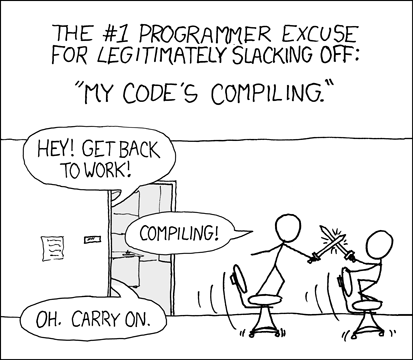
\includegraphics[height=75mm]{compiling}
  \centering
\end{frame}

\begin{frame}{Tooling}{}
  \begin{itemize}
    \item Busybox does not provide a package manager.
    \item Debian repo is more than \textbf{200G}, packaging is hard and can become messy.
    \item We need simplicity and documentation, to create infrastructure.
  \end{itemize}
  Let's build a pipeline around this to speed up our workflow.
  \flushright{\LARGE \textbf{It's all about tooling!}}
\end{frame}


\begin{frame}[fragile]{Tooling}{Build your binary}
  virtual package switch:  \mintinline{shell}{apk add -t virtual} \\
  build container \textbf{\char`~200MB}$\,\to\,$prod container
  \textbf{\char`~11MB}

  \begin{minted}{docker}
FROM alpine:3.4

ENV REPO "https://raw.githubusercontent.com/.../hello.go"
RUN apk add --no-cache -t build-dependencies go curl \
  && curl -o /tmp/hello.go "$REPO" \
  && go build -ldflags '-w -s' -o /usr/local/bin/hello /tmp/hello.go \
  && rm /tmp/hello.go \
  && apk del build-dependencies

CMD ["/usr/local/bin/hello"]
  \end{minted}
\end{frame}

\begin{frame}[fragile]{Tooling}{Build your mirror}

  \begin{block}{Murphy's law}
    Anything that can go wrong will go wrong.
  \end{block}

    \begin{itemize}
      \item Small footprint (\char`~5G)
      \item Rapid builds, offline builds
      \item Push your custom package
  \end{itemize}

  \begin{minted}{shell}
REPO_URL="rsync://${mirror}/alpine/v3.4/main/x86_64"

/usr/bin/rsync ${rsync_opts} ${REPO_URL} /tmp/alpine
/usr/bin/darkhttpd --port 8000 /tmp/alpine
  \end{minted}
\end{frame}

\begin{frame}[fragile]{Tooling}{Build your package}
  Will you recompile your dependencies at the worst moment?
  \flushright{\textbf{(no, you won't!)}}
  \\
  \begin{itemize}
    \item \textbf{abuild-keygen} generate keys. The public key has to be
      installed and shared across containers.
    \item \textbf{APKBUILD} package description file. Contains instructions for
      the package build. Based on Gentoo Linux ebuilds, an easy way to package
      is to check Archlinux AUR for examples.
    \item \textbf{abuild -r -P /your\_repo\_volume} download source, compile,
      package, push to the specified repo.
  \end{itemize}
\end{frame}

\begin{frame}[fragile]{Tooling}{Build your image}
  \begin{itemize}
    \item Build your image \\ \mintinline{text}{docker build -t my-alpine:1.0 .}
      \begin{minted}{docker}
FROM alpine:3.5
RUN echo "http://${DOCKER_BRIDGE_IP}:${PORT}" > "/etc/apk/repositories"
ADD s0m3-h4sh.rsa.pub /etc/apk/keys
      \end{minted}
    \item Start your mirror \\
      \mintinline{shell}{docker run -p 8080:${PORT} alpine-mirror}
    \item Use your pipeline!
      \begin{minted}{docker}
FROM my-alpine:1.0
RUN apk add --no-cache -t dependencies hello ...
      \end{minted}

  \end{itemize}
  \flushright{Just use \textbf{minikube} or \textbf{compose}!}

\end{frame}

\begin{frame}{Conclusion}
  \quote{
    If you think "performance" is just CPU cycles, you're very wrong.
	}{Linus Torvald}
  \quote{
    If all you have is a hammer, everything looks like a nail.
  }{Abraham Maslow}

  \begin{itemize}
    \item When building containers, think size, think network, think build time.
    \item You don't always need a full pipeline.
    \item Before starting new tools, look at what already exists.
  \end{itemize}
\end{frame}

\end{document}
